\chapter{Interacting Peers}
\label{chap:interacting-peers}

A common paradigm in concurrent programming is that of \emph{interacting
  peers}.  Several threads or processes are peers, in the sense that they
execute basically the same code.  They exchange messages to achieve some goal.
The way in which messages are exchanged can follow various patterns or
topologies.

\begin{figure}[hbtp]
%\begin{center}
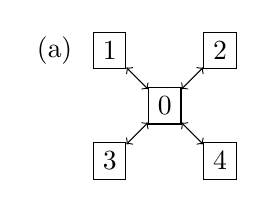
\begin{tikzpicture}[scale = 0.7]
\draw(-2,1) node {(a)};
\draw(0,0) node[draw] (0) {0};
\draw(-1,1) node[draw] (1) {1}; \draw[<->] (0) -- (1);
\draw(1,1) node[draw] (2) {2}; \draw[<->] (0) -- (2);
\draw(-1,-1) node[draw] (3) {3}; \draw[<->] (0) -- (3);
\draw(1,-1) node[draw] (4) {4}; \draw[<->] (0) -- (4);
\end{tikzpicture}
%%%%%
\hfil
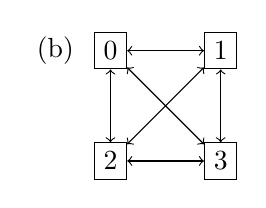
\begin{tikzpicture}[scale = 0.7]
\draw(-2,1) node {(b)};
\draw(-1,1) node[draw] (0) {0};
\draw(1,1) node[draw] (1) {1}; 
\draw(-1,-1) node[draw] (2) {2};
\draw(1,-1) node[draw] (3) {3}; 
\foreach \x in {1,...,3}  \draw[<->] (0) -- (\x);
\foreach \x in {2,...,3}  \draw[<->] (1) -- (\x);
\draw[<->] (2) -- (3);
\end{tikzpicture}
%%%%% Ring
\hfil
\def\r{1.4}
\raisebox{-1.9mm}{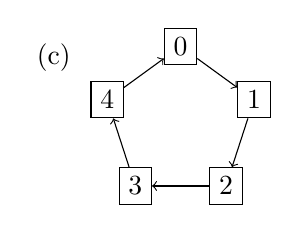
\begin{tikzpicture}[scale = 0.7]
\draw(-2.3,1.2) node {(c)};
\foreach \i in {0,...,4} 
  \draw (90-72*\i: \r) node[draw] (\i) {\i}; 
\foreach \i/\j in {0/1, 1/2, 2/3, 3/4, 4/0} \draw[->] (\i) -- (\j);
%% \draw(-1,1) node[draw] (0) {0};
%% \draw(1,1) node[draw] (1) {1}; 
%% \draw(-1,-1) node[draw] (3) {3};
%% \draw(1,-1) node[draw] (2) {2}; 
%% \draw[->] (0) -- (1); \draw[->] (1) -- (2); 
%% \draw[->] (2) -- (3); \draw[->] (3) -- (0);
\end{tikzpicture}}
%%%%% Heap
\hfil
\raisebox{-2.9mm}{
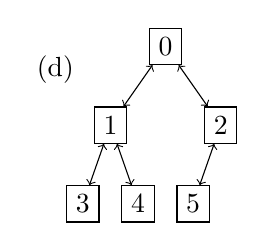
\begin{tikzpicture}[xscale = 0.7, yscale = 1.0]
\draw(-2,-0.3) node {(d)};
\draw(0,0) node[draw] (0) {0};
\draw (0)++(-1,-1) node[draw] (1) {1}; \draw[<->] (0) -- (1);
\draw (0)++(1,-1) node[draw] (2) {2}; \draw[<->] (0) -- (2);
\draw (1)++ (-0.5,-1) node[draw] (3) {3}; \draw[<->] (1) -- (3);
\draw (1)++ (0.5,-1) node[draw] (4) {4}; \draw[<->] (1) -- (4);
\draw (2)++ (-0.5,-1) node[draw] (5) {5}; \draw[<->] (2) -- (5);
% \draw (2)++ (0.5,-1) node[draw] (6) {6}; \draw[<->] (2) -- (6);
\end{tikzpicture}}%
%\end{center}
\caption{Four patterns of interacting peers: (a) a centralised pattern; (b)~a
  fully connected topology; (c) a ring; (d) a binary heap.}
\label{fig:interacting-peers}
\end{figure}

%%%%%

In this chapter we will examine four patterns of interacting peers, depicted
in Figure~\ref{fig:interacting-peers}: 
%
\begin{enumerate}
\item[(a)] A system with a centralised thread doing most of the work;

\item[(b)] A symmetric, fully connected topology, where each thread sends
  messages to all the others;

\item[(c)] A ring topology, where each thread communicates with just its two
  neighbours;

\item[(d)] A binary tree, or heap, topology, where each thread communicates
  just with its parent and two children.
\end{enumerate}
%
We will often use graph-theoretic terminology, and refer to the threads as
\emph{nodes}.  

Typically, each node will hold some data, and they want to calculate some
function of that data.  To illustrate different topologies and associated
techniques, we consider a very simple example in the first part of this
chapter: at the start, each node holds an integer; at the end, each node
should hold the sum of all those integers.
%
For each pattern, we will implement objects implementing the following trait. 
\begin{scala}
/** The trait specifying the various sum examples.
  * Each thread calls apply, passing in its value, and gets back the overall
  * sum. */
trait Sum{
  /** Submit value, and receive back overall sum. 
    * @param £me£ the identity of this thread.
    * @param £x£ the value submitted. */
  def apply(me: Int, x: Int): Int
}
\end{scala}

%%%%%

We will reason about the correctness of the patterns by identifying
\emph{invariants} that hold at certain points in the execution, for example,
about the values sent in particular messages, or properties of the state of
threads after each message that is sent or received.

We will also consider the cost of each pattern.  One obvious measure of cost
is the \emph{total} number of messages sent.  However, this isn't necessarily
a good measure of the running time if multiple messages can be sent
concurrently.
%
We will therefore also consider the number of messages sent
\emph{sequentially}.  Recall the ``happens-before'' relation $\preceq$; we say
that messages $m_1$, \ldots, $m_k$ form a \emph{totally ordered chain} if
necessarily 
\[\mstyle
m_1 \prec m_2 \prec \ldots \prec m_k,
\]
i.e., those messages have to be sent in that sequential order.  We will be
interested in identifying the length of the longest totally ordered chain, and
how that relates to the number of threads.

In the latter part of this chapter, we will consider a more sophisticated
problem for a ring topology, namely to elect one of the nodes as a leader. 

%%%%%%%%%%%%%%%%%%%%%%%%%%%%%%%%%%%%%%%%%%%%%%%%%%%%%%%%%%%%

\section{Centralised Pattern}

We start with the centralised pattern: see Figure~\ref{fig:sum-centralised}.
In this protocol, each client node sends its value to a central node, with
identity~|0|.  The controller calculates the sum, and sends the sum back.
We use a single channel in each direction, which is shared by the client
nodes.  This pattern has similarities with the client-server pattern we
studied in Chapter~\ref{chap:clientServer}, except the controller has its own
value. 

%%%%%

\begin{figure}
\begin{scala}
/** Implementation of £Sum£ using a controller.  The controller is the node
  * with identity £0£. */
class Centralised(n: Int) extends Sum{
  private val toController = new BuffChan[Int](n-1 max 1)
  private val fromController = new BuffChan[Int](n-1 max 1)

  def apply(me: Int, x: Int): Int = {
    if(me == 0){ // This is the controller.
      var sum = x
      // Receive values from other threads.
      for(i <- 1 until n){ val w = toController?(); sum += w }
      // Distribute sum.
      for(i <- 1 until n) fromController!sum
      sum
    }
    else{
      toController!x     // Submit my value.
      fromController?() // Get back the result.
    }
  }
}
\end{scala}
\caption{The sum example using the centralised pattern.}
\label{fig:sum-centralised}
\end{figure}

%%%%%

Arguing for the correctness of this program is straightforward.
Write $x_i$ for the value chosen by node~$i$.  Then during the first stage of
the protocol, the following invariant holds for the controller:
%
\begin{eqnarray*}
\sm{sum} & = & 
   x_0 + \sum \set{x_i \| 1 \le i < \sm n \land 
           \mbox{node~$i$'s value has been received}}.
\end{eqnarray*}
%
At the end of the |for| loop, the controller has received all the values, so
|sum| holds the desired result. 

\begin{instruction}
Make sure you understand the details of this program and the correctness
argument.
\end{instruction}

%%%%%

We can test the program, and the ones in subsequent sections, against
a sequential specification.  We arrange for each thread to pick a random value
for~|x|, write it into a global array~|xs| (indexed by thread identities, to
avoid race conditions), use the |Sum| object to obtain the purported sum, and
write it to a global array~|results| (again indexed by thread identities).  We
then calculate the correct sum sequentially (as |xs.sum|) and check that each
element of |results| is as expected.

%%%%%

This protocol uses $2(\sm n-1)$ messages in total: each client thread sends one
message and receives one message.  However, none of these messages can occur
concurrently, since all messages involve the controller.
Write $\sm{toController}.i$ for the communication on |toController| from
thread~$i$, and similarly for |fromController|.
We can find a totally-ordered chain of communications:
\[
\begin{align}
\mbox{\SCALA{toController}}.i_1 \prec \mbox{\SCALA{toController}}.i_2 
  \prec \ldots  \prec \mbox{\SCALA{toController}}.i_{\ss n-1} \prec \\
\qquad
  \mbox{\SCALA{fromController}}.j_1 \prec \mbox{\SCALA{fromController}}.j_2 
  \prec \ldots \mbox{\SCALA{fromController}}.j_{\ss n-1}
\end{align}
\]
for some permutations $i_1, \ldots, i_{\ss n-1}$ and $j_1, \ldots, j_{\ss
  n-1}$ of $1, \ldots, \sm n-1$.


%%%%%%%%%%%%%%%%%%%%%%%%%%%%%%%%%%%%%%%%%%%%%%%%%%%%%%%

\section{Fully Connected Pattern}

We now consider the fully connected pattern: see
Figure~\ref{fig:sum-symmetric}.  In this solution, each node sends its value
to every other node, and each node calculates the sum using the values it
receives.

%%%%%

\begin{figure}[htbp]
\begin{scala}
/** Implementation of £Sum£ using the symmetric (fully connected) pattern. */
class Symmetric(n: Int) extends Sum{
  /** Channels to send to nodes, indexed by the receivers' identities. */
  private val toNode = Array.fill(n)(new BuffChan[Int](n-1 max 1))

  def apply(me: Int, x: Int): Int = {
    for(i <- 0 until n) if(i != me) toNode(i)!x }
    // Receive values.
    var sum = x // Sum so far.
    for(i <- 1 until n){ val w = toNode(me)?(); sum += w }
    sum
  }
}
\end{scala}
\caption{The sum example using a fully connected topology.}
\label{fig:sum-symmetric}
\end{figure}

%%%%%

Each node needs to send $\sm{n}-1$ messages, and receive $\sm{n}-1$ messages.
We give each node its own channel on which it can receive messages.  We
arrange for the two stages to be performed sequentially.  However, in order to
avoid deadlocks, we need to make the channels buffered with capacity (at
least) |n-1|, so all the threads can send before any is ready to receive (when
$\sm n = 1$, we give the channels capacity~$1$, because the capacity fo a
|BuffChan| must be strictly positive).  Alternatively, we could have run the
two stages concurrently, using a separate thread for each, in which case we
could have used synchronous channels.

Write $x_j$ for the value chosen by node~$j$.  Then during the receiving loop,
each node~$i$ has a value for \SCALA{sum} such that:
%
\begin{eqnarray*}
\sm{sum} & = & 
  x_i + \sum \set{x_j \| \mbox{node~$j$'s value has been received by node~$i$}}.
\end{eqnarray*}
%
Each node sends to each other node; and each node receives exactly $\sm n-1$
times; hence each node must receive each other node's value.  This means that
each node's final value for |sum| is the correct sum.

\begin{instruction}
Make sure you understand the details of the code and the correctness
argument.
\end{instruction}

%%%%%

The above program suffers from contention.  
Each \SCALA{sender} sends to the other nodes in order, starting from
\SCALA{0}.  This means that:
%
\begin{itemize}
\item
Initially, all the nodes are contending to send to node~\SCALA{0}, so most
will be temporarily blocked;

\item
Node $\sm n-1$ has to wait until another node has finished sending to
\emph{all} other nodes before receiving \emph{anything}.  %% This gives a chain
%% of length $2\sm{n}-3$ ($\sm n-2$ sends before this node receives anything,
%% and then $\sm n-1$ receives by this node).
\end{itemize}

A better approach is for each node to send in a different order, say starting
from the one with identity one higher than itself:
%
\begin{scala}
  for(i <- 1 until n) toNode((me+i)%n)!x 
\end{scala}
%
If all the nodes proceed at the same speed, this is likely to avoid contention
for the channels.  Of course, unfortunately scheduling might create
contention; but this seems unlikely. 

%%%%%

This protocol uses $\sm n(\sm n-1)$ messages in total, with sequential chains
of length~$2(\sm n -1)$.  The $O(\sm n^2)$ total number of messages means that
a fully connected topology has rather a large communication overhead: each of
the other patterns uses fewer messages. 
 % intro, centralised, fully-connected
\section{A Ring Topology}

A common way to coordinate multiple threads is via a ring, where each thread
communicates with just its two neighbours (see
Figure~\ref{fig:interacting-peers}(c)).  A ring may be either
\emph{unidirectional}, where messages go only one way round the ring, or
\emph{bidirectional}, where messages can go both ways round the ring.  It is
common to use the word \emph{token} for a message sent in a ring.

Rings are particularly common in distributed systems, where several nearby
computers are physically wired into a ring.  However, our examples in this
chapter will consider nodes in a \emph{logical} ring.  

We will see two protocols for the sum example using a unidirectional ring with
|n| nodes, where each node~$i$ sends messages to node $(i+1) \bmod \sm n$ and
receives from node $(i-1) \bmod \sm n$ (so messages are sent clockwise in
Figure~\ref{fig:interacting-peers}(c)).  In the first protocol, a single token
is passed twice round the ring.  In the second protocol, |n| tokens are
simultaneously passed round the ring.

%%%%%%%%%%

\subsection{The First Ring Protocol}

The first protocol uses two stages.  During the first stage, node~\SCALA{0}
acts as the initiator, by sending a token containing its value.  Each node in
turn receives the token, which contains the sum so far, calculates the new
sum, including its own value, and sends it on.  More precisely, letting $x_j$
be the initial value for node~$j$, the value passed from node $i$ to
node~$(i+1) \bmod n$ equals:
%
\[\mstyle
\sum \set{x_j \| 0 \le j \le i}.
\]
When the value gets back to node \SCALA{0} it equals the overall sum, 
\[\mstyle
\sum \set{x_j \| 0 \le j \le \sm n-1}.
\]
This value is then passed around the ring in the second stage, and each node
returns this value.

%%%%%

\begin{figure}
\begin{scala}
/** Implementation of £Sum£ using a ring, with a distinguished initiator.
  * The initiator is the thread with identity £0£. */
class Ring(n: Int) extends Sum{
  require(n >= 2)

  /** Channels connecting the nodes.  Channel £chan($i$)£ goes from node
    * £$(i-1)\bmod \sm n$£ to node £$i$£; so node £$i$£ receives on £chan($i$)£ and sends
    * on £chan($(i+1)\bmod \sm n$)£. */
  private val chan = Array.fill(n)(new SyncChan[Int])
 
  def apply(me: Int, x: Int): Int = {
    val in = chan(me); val out = chan((me+1)%n)
    if(me == 0){                  // This is the initiator.
      out!x                       // Start the communications going.
      val sum = in?()             // Receive sum back.
      out!sum                     // Send it round.
      sum
    }
    else{
      val sum1 = in?()            // Receive sum so far.
      out!sum1+x                  // Pass on updated values.
      val sum = in?()             // Receive final sum.
      if(me != n-1) out!sum   // Pass it on.
      sum
    }
  } 
}
\end{scala}
\caption{The sum example using a ring topology with a single token.}
\label{fig:sum-ring1}
\end{figure}

%%%%%

The program is in Figure~\ref{fig:sum-ring1}.  We use an array |chan| of
channels, where channel |chan(|$i$|)| connects node~$(i-1)\bmod \sm n$ to
node~$i$.  This means that node~$i$ receives on |chan(|$i$|)| and sends on
|chan(|$(i+1)\bmod \sm n$|)|.  It is always a good idea to be clear about how
arrays of channels are indexed.  The code for each node starts by defining the
names |in| and |out| for the relevant channels: this is good practice, as it
makes the subsequent code far clearer.

The code is then fairly straightforward, and explained by comments.  One small
optimisation is that in the second stage, node~$\sm n - 1$ does not send the
token back to node~$0$, since there is no need.
%
\begin{instruction}
Study the details of the code. 
\end{instruction}

This protocol uses $2\sm n-1$ messages, sent sequentially.  Each node is
inactive for most of the time.  This pattern is most effective for problems
where each node can do computation between sending a message and receiving the
next. 


%%%%%%%%%%%%%%%%%%%%%%%%%%%%%%%%%%%%%%%%%%%%%%%%%%%%%%%%%%%%

\subsection{The Second Ring Protocol}

We now consider the second ring protocol.  All the values are passed round the
ring concurrently in separate tokens.  Thus each node sees all the values, so
can calculate the maximum. 

More precisely, on its $k$th iteration, each node~$i$ receives a value
from node~$(i-1) \bmod \sm n$ that originated with node $(i-k)\bmod \sm n$; it
sends this value on to node~$(i+1)\bmod \sm n$, and keeps track of the
sum, \SCALA{sum}, it has seen so far:
%
\begin{eqnarray*}
\sm{sum} & = & \sum \set{x_{(i-j)\bmod \ss n} \| 0 \le j \le k}.
\end{eqnarray*}
%
At the end of iteration~$\sm n-1$, it holds the overall sum.

%%%%%

\begin{figure}
\begin{scala}
/** Implementation of £Sum£ using a symmetric ring. */
class RingSym(n: Int) extends Sum{
  /** Channels connecting the nodes.  Channel £chan($i$)£ goes from node
    * £$(i-1)\bmod \sm n$£ to node £$i$£; so node £$i$£ receives on £chan($i$)£ and sends
    * on £chan($(i+1)\bmod \sm n$)£.  These channels need to be buffered. */
  private val chan = Array.fill(n)(new OnePlaceBuffChan[Int])

  def apply(me: Int, x: Int): Int = {
    val in = chan(me); val out = chan((me+1)%n)
    var sum = x
    out!x                 // Send my value round.
    for(k <- 1 until n){
      val w = in?()       // Receive next value.
      sum += w
      out!w               // Pass it on.
    }
    val w = in?(); assert(x == w) // Receive my value back.
    sum
  }
\end{scala}
\caption{The sum example using a ring topology with multiple tokens.}
\label{fig:sum-ring2}
\end{figure}

%%%%%

The code is in Figure~\ref{fig:sum-ring2}.  The channels are indexed as for
the previous ring protocol.  However, it is necessary to use buffered channels
in this case: each node starts by sending, so if we used synchronous channels,
there would be an immediate deadlock.  We use one-place buffered channels;
however, a bit more buffering might help to overcome inconsistencies in speeds
of nodes.

\begin{instruction}
Study the details of the code, and check the properties claimed above.
\end{instruction}

This protocol uses a total of $\sm n^2$ messages, so considerably more than
the previous protocol.  (We could omit the final message sent by each node, to
reduce this to $\sm n(\sm n - 1)$.)  However, it uses only |n| rounds,
compared with $2\sm n-1$ for the previous protocol.  Each node is active for
most of the time (so one slow node will slow down the whole ring).

%%%%%%%%%%%%%%%%%%%%%%%%%%%%%%%%%%%%%%%%%%%%%%%%%%%%%%%%%%%%

\section{Heap-Based Protocol}

The final protocol works by arranging nodes into a binary tree.  In the
initial stage, values get passed up the tree, starting from the leaves: each
node passes to its parent the sum of the subtree for which it is the root.  At
the end of this stage, the root of the tree obtains the overall sum.  In the
second stage, this sum is passed back down the tree.

More precisely, we arrange the nodes into a binary \emph{heap}: see
Figure~\ref{fig:interacting-peers}(d).  Node~$0$ is the root of the tree.
Node~$i$ is the parent of nodes $2i+1$ and $2i+2$ (if those nodes exist).


%% \begin{center}
%% \begin{tikzpicture}[xscale = 0.8, yscale = 1.0]
%% \draw(0,0) node[draw] (0) {0};
%% \draw (0)++(-1.2,-1) node[draw] (1) {1}; \draw[<->] (0) -- (1);
%% \draw (0)++(1.2,-1) node[draw] (2) {2}; \draw[<->] (0) -- (2);
%% \draw (1)++ (-0.7,-1) node[draw] (3) {3}; \draw[<->] (1) -- (3);
%% \draw (1)++ (0.7,-1) node[draw] (4) {4}; \draw[<->] (1) -- (4);
%% \draw (2)++ (-0.7,-1) node[draw] (5) {5}; \draw[<->] (2) -- (5);
%% \draw (2)++ (0.7,-1) node[draw] (6) {6}; \draw[<->] (2) -- (6);
%% \draw (3)++ (-0.35,-1) node[draw] (7) {7}; \draw[<->] (3) -- (7);
%% \draw (3)++ (0.35,-1) node[draw] (8) {8}; \draw[<->] (3) -- (8);
%% \draw (4)++ (-0.35,-1) node[draw] (9) {9}; \draw[<->] (4) -- (9);
%% \end{tikzpicture}
%% \end{center}

%%%%%

The code is in Figure~\ref{fig:sum-tree}.  We use two arrays of channels, |up|
and |down| to pass data up and down the tree.  The arrays are indexed by the
\emph{child} node: \SCALA{up(i)} and \SCALA{down(i)} are used to communicate
between node~$i$ and its parent, node~$(i-1) \div 2$.

\begin{instruction}
Study the details of the definition of a node. 
\end{instruction}

%%%%%

\begin{figure}[bht]
\begin{scala}
class Tree(n: Int) extends Sum{
  /** Channels leading up and down the tree.  Each array is indexed by
    * the child's identity. */
  private val up, down = Array.fill(n)(new SyncChan[Int])
  
  def apply(me: Int, x: Int) = {
    val child1 = 2*me+1; val child2 = 2*me+2  // Identities of children.
    var sum = x                                     // Sum seen so far.
    // Receive sub-sums from both children.
    if(child1 < n){ val sum1 = up(child1)?(); sum += sum1 }
    if(child2 < n){ val sum2 = up(child2)?(); sum += sum2 }
    // £sum£ is the sum of values for the subtree rooted at me.
    // Send £sum£ to parent, and wait for overall sum.
    if(me != 0){ up(me)!sum; sum = down(me)?() }
    // Send £sum£ to children.
    if(child1 < n) down(child1)!sum
    if(child2 < n) down(child2)!sum
    sum
  }
}
\end{scala}
\caption{The tree-based protocol.}
\label{fig:sum-tree}
\end{figure}

%%%%%

Each node starts by defining names |child1| and |child2| for the indices of
its two children, if they exist.  Again, this is good practice, as it makes
the subsequent code clearer.  As an aside, it is easy to get the indexing
wrong in such cases: I recommend drawing a picture like that in
Figure~\ref{fig:interacting-peers}(d).  

The node receives values from its two
children, if those children exist, i.e.~they have identities less than~|n|.
The values received will be the subtotals for the two subtrees; so adding
these values to the node's own value gives the subtotal for the tree rooted at
this node.  The node then passes this value to its parent, if this is not the
root.  It then waits to receive back a value from its parent (again, if this
is not the root), which it passes down to its children.

\begin{instruction}
Study the code.  In particular, consider the different steps taken by leaf
nodes, internal nodes, and the root.
\end{instruction}

%%%%%

We now justify the correctness of the protocol, by formalising the claim we
made above.  We write $decendents(i)$ for the indices of the nodes in the
subtree rooted at~$i$:
%
\begin{eqnarray*}
descendents(i) & = & 
  \set{i} 
    \begin{align}
      \null \union (\If 2i+1 < \sm n \mbox{ then } descendents(2i+1) 
      \mbox{ else } \set{}) \\
      \null \union
      (\If 2i+2 < \sm n  \mbox{ then }  descendents(2i+2) \mbox{ else } \set{}).
    \end{align}
\end{eqnarray*}
%
Then we claim that each node~$i$ with $0 < i < \sm n$ passes to its parent the
sum of the values held by the nodes in the subtree rooted at~$i$, that is:
%
\[\mstyle
\sum \set{x_j \| j \in descendents(i)}
\]
The claim can be proven by induction on the size of $descendents(i)$, as
follows.
%
\begin{itemize}
\item
Consider the case where $2i + 2 < \sm n$, so node~$i$ has two children.  Then
\[
\begin{array}{cl}
& \displaystyle\sum \set{x_j \| j \in descendents(i)}  \\
= & \qquad\mbox{(expanding the definition of $descendents(i)$)} \\

& \displaystyle\sum 
  \set{x_j \mid j \in \set{i} \union  descendents(2i+1) \union
               descendents(2i+2) } \\
= & \qquad\mbox{(addition is associative)} \\ 
& x_i 
  \begin{align}
  \null + \displaystyle \sum \set{x_j \| j \in descendents(2i+1)} \\
  \null + \displaystyle \sum \set{x_j \| j \in descendents(2i+2)}.
  \end{align}
\end{array}
\]
By the inductive hypothesis, the second term is the value received from
$\sm{child1} = 2i+1$, and the third term is the value received from
$\sm{child2} = 2i+2$.  Hence the above value equals the value that node~$i$
passes to its parent, as required.

\item
The cases where node~$i$ has one or no children are similar.
\end{itemize}
%
Hence, we can deduce that node~$0$ ends up with the overall sum, which is
passed back down the tree.

This protocol uses $2(\sm n-1)$ messages (each node except~0 sends one message
on its \SCALA{up} channel, and receives one message on its \SCALA{down}
channel).  There are four messages between each internal node and its
children, so the total number of rounds is about $4\lfloor \log \sm n \rfloor$
rounds, i.e.~about $4$ times the height of the tree.  This is the most
efficient of the patterns we have seen, so we will use the tree pattern again
in later chapters.
 % rings and heaps
\section{Leadership Election in a Ring}

We now consider a different problem based on a ring.  Suppose we have |n|
nodes arranged in a unidirectional ring, each of which has a unique identity.
However, the nodes do not know what |n| is, and the identities might not be in
the range $\interval{0}{\sm n}$.  This might be the case in a distributed
system, where the identities are MAC addresses or IP addresses.  Further, each
node has ports with which it communicates with its neighbours in the ring.

We want a protocol to elect one node as a leader (or controller) for
subsequent computation.  More precisely, each node should end up with a
boolean indicating whether it is the leader: the leader could then inform the
others of its own identity, if that is required.  We will encapsulate
solutions into classes with the following interface.
%
\begin{scala}
trait LeadershipElection{
  /** Run the protocol using identity £id£, receiving messages on £in£, and sending 
    * on £out£.  Return a £Boolean£ indicating whether this node is the leader. */
  def apply(id: Int, in: ??[Int], out: !![Int]): Boolean
}
\end{scala}
%

We will consider two protocols for this problem. 
Note that there is no way to adapt the first ring protocol for the sum
problem, because there is no way to decide who should initiate the protocol:
this would requires that we already have a leader! 

%%%%%%%%%%%%%%%%%%%%%%%%%%%%%%%%%%%%%%%%%%%%%%%%%%%%%%%

Instead, we consider a simple adaptation of the second ring protocol for the
sum protocol.  We identify the node with the maximum identity, and it becomes
leader.  The code is in Figure~\ref{fig:leadership1}.  Each identity is passed
round the ring.  Each node keeps track, in variable |max|, of the maximum
identity it has seen.  When it receives back its own identity, it can deduce
that it has seen all the identities, and so is done.  It is the leader if
|max| equals its own identity.

%%%%%

\begin{figure}[htbp]
\begin{scala}
class SimpleLeaderRing extends LeadershipElection{
  def apply(id: Int, in: ??[Int], out: !![Int]): Boolean = {
    var max = id; var done = false; out!id
    while(!done){
      val x = in?()
      if(x > max) max = x
      else if(x == id) done = true
      if(!done) out!x    
    }
    max == id
  }
}
\end{scala}
\caption{The first leadership election protocol.}
\label{fig:leadership1}
\end{figure}

%%%%%

\begin{instruction}
Study the details of the implementation.
\end{instruction}

Every node sees every identity, so this protocol uses $\sm n^2$ messages, sent
in |n|~rounds. 


%%%%%%%%%%%%%%%%%%%%%%%%%%%%%%%%%%%%%%%%%%%%%%%%%%%%%%%

The second protocol, due to Peterson~\cite{peterson-election}, is more
efficient.  It reduces the total number of messages to $O(\sm n \log \sm n)$.
For simplicity, we assume that all the identities are non-negative.

%%%%%

\begin{figure}
\begin{scala}
/** The Peterson Leadership Election protocol. 
  * This implementation assumes all identities are non-negative. */
class PetersonLeader extends LeadershipElection{
  def apply(id: Int, in: ??[Int], out: !![Int]): Boolean = {
    var relaying = false; var leader = false; var tid = id
    while(!leader && !relaying){
      out!tid; val x = in?()
      if(x == tid){ out!(-1); leader = true }
      else{
        out!x; val y = in?()
        if(x > tid && x > y) tid = x
        else relaying = true
      }
    }
    // Relaying.
    while(relaying){
      val x = in?(); out!x
      if(x < 0) relaying = false
    }
    leader
  }
}
\end{scala}
\caption{The Peterson leadership election protocol.}
\label{fig:leadership2}
\end{figure}

%%%%%

The code is in Figure~\ref{fig:leadership2}.  In each round, some of the node
are \emph{active}, and the remainder are \emph{relaying}: the active nodes are
ones that are still candidates to become the election, while those relaying
simply pass on messages.  Initially all nodes are active.  Each active node
has a \emph{temporary identity}~|tid|: this is one of the original identities,
but each node's temporary identity changes from round to round.

In each round, each active node sends its temporary identity on the ring.  If
a node then receives back its own temporary identity, it must be the only
active node, and so becomes the leader.  It passes a negative value round the
ring to signal to the other nodes that the protocol is complete (this is why
we assumed non-negative identities; an alternative would be to change the type
of the channels, and to use a different subtype for the termination messages).

If there are more than two active nodes, each temporary identity is passed
forward to two other active nodes: thus each active node sees the temporary
identities~|x| and |y| of the first two active nodes upstream from it.  If the
first of these temporary identities, |x|, is larger than the other, and also
larger than the node's temporary identity, then this node remains active,
adopting |x| as its new temporary identity.  Otherwise, the node becomes a
relayer.



\begin{instruction}
Study the details of the code.
\end{instruction}

We now justify the correctness of this protocol.  We start with the safety
property that, assuming the protocol terminates, a single node returns |true|
to indicate that it is the leader.  First, note that the largest initial
identity survives each round: only smaller identities are eliminated.  Next,
note that on each round, the active nodes have distinct temporary identities:
if a temporary identity survives a round, it is adopted by the next downstream
active node.  Thus, if an active node receives back its own temporary
identity, it must indeed be the only active node, and its temporary identity
is the maximum of the initial identities.  Hence, if the protocol terminates,
a single node returns |true|.

We now show that the protocol does indeed terminate (a liveness property), and
justify the earlier claim about the number of messages.  Consider a particular
round, other than the final round; and consider three consecutive active
nodes, $n_0$, $n_1$ and~$n_2$, in downstream order, with temporary identities
$tid_0$, $tid_1$ and~$tid_2$, respectively.  Suppose $n_2$ remains active
after this round; then we must have $tid_1 > tid_0$ (since these values
instantiate $n_2$'s |x| and |y| variables).  But $n_1$ receives $tid_0$ for
its |x| variable, and $tid_1$ was its previous temporary identity, so $n_1$
becomes a relayer.

Hence, in each round (except the final round), out of any two consecutive
active nodes, at least one becomes a relayer.  This means that the number of
active nodes is reduced by at least a half in each round.  Hence the protocol
terminates in at most $1 + \lfloor \log \sm n \rfloor$ rounds.

On each round, every node sends and receives two messages: this is obviously
true of the active nodes; and the relayers simply receive and send the
messages sent by the closest upstream active node.  Hence $2 \sm n$ messages
are sent on each round, and so the total number of messages is $O(\sm n \log
\sm n)$.
 % leadership election in a ring.
\section{Building a spanning tree}

Suppose we have a collection of nodes in a graph.  Some, but not necessarily
all, pairs of nodes are directly connected: there are channels between the two
nodes in each direction.  It might be that the graph is disconnected: it might
not be possible to find a path from one node to another.  

One of the nodes is designated as a controller.  We want to find which other
nodes are reachable from the controller, and to find a spanning tree for them,
i.e.~a collection of edges that connect those nodes, without any cycles.  This
spanning tree could be used subsequently to distribute messages.

The idea of the protocol is as follows.  Initially, node~|0| sends a message
|Start(0)| to each of its neighbours.  For each such neighbour~|n|, if this is
the first |Start| message it has seen, then the edge from~|0| to~|n| will be
included in the spanning tree.  In this case, node~|n| tries to continue the
tree by sending a message |Start(n)| to each of its neighbours, except~|0|,
which react in a similar way.  However, if a node receives two or more |Start|
messages, it sends a reply |No| to all except the first, so the corresponding
edge will not be part of the spanning tree.  

Suppose node~|p| sends a |Start| message to node~|n|, and this is node |n|'s
first |Start| message, then |n| will eventually return to~|p| a message of the
form |Finished(edges)|, where |edges| represents a tree, starting with an edge
from~|p| to~|n|, and maybe including subsequent nodes from there.  Node~|p|
can accumulate the edges from all such messages it receives, and return the
result to its predecessor in the spanning tree. 


\begin{figure}
\begin{scala}
import scala.collection.mutable.ArrayBuffer

/** adjacency should be symmetric and irreflexive. */ 
class SpanningTree(n: Int, adjacency: Array[Array[Boolean]]){
  require(adjacency.length == n && adjacency.forall(_.length == n))

  private type NodeId = Int
  private type Edge = (NodeId,NodeId)

  private trait Msg
  /** A message from `prev` telling the recipient to start exploration. */
  private case class Start(prev: NodeId) extends Msg
  /** A message indicating that the sender has constructed a subtree using
    * `edges`. */
  private case class Finished(edges: List[Edge]) extends Msg
  /** Message indicating that the relevant edge should not be included. */
  private case object No extends Msg

  private var result: List[Edge] = null

  private val chans = Array.ofDim[BuffChanT[Msg]](n,n)

  private val verbose = false 

  private def node(me: Int, ins: Array[??[Msg]], outs: Array[!![Msg]]) = ...

  def apply(): List[Edge] = ...
}
\end{scala}
\caption{Outline of the spanning tree code.}
\label{fig:spanning-tree}
\end{figure}

%%%%%%%%%%

A node with identity `me`.  The channels in `ins` and `outs` connect this
node with its neighbours, with `ins(i)` and `outs(i)` connecting to the
same neighbour. 

\begin{figure}
\begin{scala}
  private def node(me: Int, ins: Array[??[Msg]], outs: Array[!![Msg]]) 
  = thread(s"node($me)"){
    val size = ins.length; require(outs.length == size); var edges = List[Edge]()
    if(size != 0){
      // Identity of this node's predecessor, and its index in the arrays.
      var prev = -1; var pIx = -1; var terminated = false
      // Waiting phase
      if(me != 0) attempt{
        alt(| ( 
          for(i <- 0 until size)
          yield ins(i) =?=> { case Start(p) => prev = p; pIx = i }
        ) )
      }{ terminated = true }
      if(!terminated){
        // Sending phase
        for(i <- 0 until size; if i != pIx) outs(i)!Start(me)
        // Receiving phase
        val pendingIn = Array.fill(size)(true); if(pIx >= 0) pendingIn(pIx) = false
        serve(| (
          for(i <- 0 until size)
          yield pendingIn(i) && ins(i) =?=> { m =>
            m match{
              case Finished(es) => edges = es++edges
              case Start(_) => outs(i)!No
              case No =>
            }
            pendingIn(i) = false
          }
        ) ) // end of serve
        // Finishing phase
        if(pIx >= 0) outs(pIx)!Finished((prev,me)::edges)
      } // end of if(!terminated)
    } // end of if(ins.nonEmpty)
    if(me == 0){
      result = edges
      for(i <- 0 until n; j <- 0 until n){
        val c = chans(i)(j); if(c != null) c.close()
      }
    } 
  }
\end{scala}
\caption{A node in the spanning tree example.}
\label{fig:spanning-tree-node}
\end{figure}

%%%%%%%%%%

\begin{figure}
\begin{scala}
  import scala.collection.mutable.ArrayBuffer

  def apply(): List[Edge] = {
    // Initialise channels
    // chans(i)(j) is from i to j
    for(i <- 0 until n; j <- 0 until n; if adjacency(i)(j)){
      assert(i != j && adjacency(j)(i))
      chans(i)(j) = new BuffChan[Msg](2)
    }
    // In-ports for node i.
    def mkIns(i: NodeId): Array[??[Msg]] = {
      val ins1 = new ArrayBuffer[??[Msg]]
      for(j <- 0 until n; if adjacency(i)(j)) ins1 += chans(j)(i)
      ins1.toArray
    }
    // Out-ports for node i.
    def mkOuts(i: NodeId): Array[!![Msg]] = {
      val outs1 = new ArrayBuffer[!![Msg]]
      for(j <- 0 until n; if adjacency(i)(j)) outs1 += chans(i)(j)
      outs1.toArray
    }
    run(|| (for(i <- 0 until n) yield node(i, mkIns(i), mkOuts(i))))
    result
  }
\end{scala}
\caption{The main code for the spanning tree example.}
\label{fig:spanning-tree-apply}
\end{figure}

%%%%%%%%%%

\begin{figure}
\begin{scala}
  def doTest = {
    val n = 5+Random.nextInt(5)
    val adjacency = Array.ofDim[Boolean](n,n)
    for(i <- 0 until n; j <- 0 until i; if Random.nextDouble() <= 0.3){ 
      adjacency(i)(j) = true; adjacency(j)(i) = true 
    }
    // println(adjacency.map(_.mkString(", ")).mkString("\n"))
    val tree = new SpanningTree(n, adjacency)()

    // Check adjacency and result compatible
    def errMsg = adjacency.map(_.mkString(", ")).mkString("\n")+"\n"+tree
    // Nodes reached by the tree
    val reached = new Array[Boolean](n); reached(0) = true
    for((a,b) <- tree){
      assert(reached(a), s"Unreached source of edge: ($a, $b)\n"+errMsg)
      assert(adjacency(a)(b), s"Non-edge used: ($a, $b)\n"+errMsg) 
      reached(b) = true
    }
    // Count number reached
    var numReached = 0; for(i <- 0 until n; if reached(i)) numReached += 1
    // Does `tree` have the right length to be a tree?
    assert(numReached == tree.length + 1, s"Not a tree.\n"+errMsg)
    // Check no other node should have been reached.
    for(i <- 0 until n; if !reached(i); j <- 0 until n)
      assert(!(reached(j) && adjacency(i)(j)), s"$i not reached:\n"+errMsg)
  }
\end{scala}
\caption{Testing the spanning code example.}
\label{fig:spanning-tree-test}
\end{figure}
 % building a spanning tree.

%%%%%%%%%%%%%%%%%%%%%%%%%%%%%%%%%%%%%%%%%%%%%%%%%%%%%%%%%%%%

\section{Summary}

In this chapter, we have studied the idea of interacting peers, where a number
of threads or processes, executing basically the same code, work together to
achieve some goal.  The peers can be connected together via various
topologies, including a centralised topology, a fully connected topology, a
ring, a binary tree.  In the centralised topology,
the central controller can be a bottleneck.  In the fully connected topology,
the number of messages grows quadratically with the number of nodes, which
might be excessive.  Rings can be effective in a number of situations.  A
binary tree is often a particularly efficient topology, allowing many problems
to be solved in time $O(\log n)$ for $n$ nodes.

We illustrated each of the topologies by using them to find the sum of
values initially held by the nodes.  This generalises to allow the data to be
combined together in different ways: Exercise~\ref{ex:ringFold} investigates
this for the case of a ring.
%% easily: given an
%% associative, commutative function~$f$, we can use these patterns to calculate
%% \[\mstyle
%% f(f( \ldots f (f( f(x_0, x_1), x_2), x_3), \ldots), x_{n-1})
%% \]
%% where $x_0,\ldots,x_{n-1}$ are the data values. 
We reasoned about the different programs by identifying \emph{invariants}:
properties that were true at key points in the program, for example at the end
of each iteration. 

We also considered another problem for a ring topology, namely that of
leadership election.  A straightforward algorithm solves this problem in using
$O(n^2)$ messages for $n$ nodes  The more sophisticated Peterson algorithm
solves it using $O(n \log n)$ messages, by eliminating at least half the
candidates on each round.

Finally, we considered the problem of finding a spanning tree of edges in a
general graph. 


%%%%%%%%%%%%%%%%%%%%%%%%%%%%%%%%%%%%%%%%%%%%%%%%%%%%%%%

\exercises


\begin{question}
\label{ex:ringFold}
Suppose $n$ threads are connected in a ring.  Each thread~$i$ (for $i = 0,
\ldots, n-1$) initially holds a value~$x_i: T$.  Write a concurrent program so
that each thread ends up in possession of the value
\[\mstyle
f(f(f(\ldots f(x_0, x_1), x_2) \ldots ), x_{n-1}),
\]
for some given function $f$.
%% ; or using functional programming notation:
%% \[
%% \mathrm{foldl1}~f~ List(x_0, x_1, \ldots, x_{n-1})
%% \]
Give your program the following signature (where $\sm{xs}(i) = x_i$, for
each~$i$):
%
\begin{mysamepage}
\begin{scala}
class RingFold[T](xs: Array[T], f: (T,T) => T, outs: Array[SyncChan[T]]){  
  private val n = xs.length
  require(n >= 2 && outs.length == n)

  def apply(): ThreadGroup = ...
}
\end{scala}
\end{mysamepage}
%
\noindent
Or, if you use buffered channels of type |BuffChan|, you will need to write 
\begin{scala}
class RingFold1[T: scala.reflect.ClassTag] ...
\end{scala}
%
Each thread should output its final result on the appropriate |outs| channel.
You should state properties that hold at key points of your program, for
example concerning the values passed on channels.

Test your code. 

What property of~$f$ will allow a different program that achieves the same
goal?  Explain your answer, and outline how this can be achieved.  (A full
implementation is not necessary.)
\end{question}

%%%%%

\begin{answerI}
This is a polymorphic generalisation of the sum example from the body of the
book. 

We write $x_i$ for $\sm{xs}(i)$.  Define
\[\mstyle
\mathrm{combine}~f~ \seq{x_0, x_1, x_2, \ldots, x_k} = 
  f(f(f(\ldots f(x_0, x_1), x_2) \ldots ), x_k),
\]
i.e.,~those elements combined together using~$f$.  

My code is below.  A single token is passed twice round the ring.  On the
first cycle, the desired value is built up.  The node with identity~$me$ sends
$\mathrm{combine}~f~\seq{x_0, x_1, x_2, \ldots, x_{me}}$.  This is easily
proven by induction, and is justified by the comments in the code.  The
comment concerning |y| holds because the value received was sent by
node~$\sm{me}-1$, which is running the same protocol.  Hence
node~0 receives back the desired result, which then gets past round the ring
on the second cycle.
%
\begin{scala}
class RingFold[T](xs: Array[T], f: (T,T) => T, outs: Array[SyncChan[T]]){
  private val n = xs.length
  require(n >= 2 && outs.length == n)

  /** The channels connecting nodes, indexed by the recipient's identity:
    * node(i) receives on chans(i) and sends on chans((i+1)%n). */
  private val chans = Array.fill(n)(new SyncChan[T]) 

  /** A single node. */
  private def node[T](me: Int) = thread{
    val left = chans(me); val right = chans((me+1)%n)
    val out = outs(me); val x = xs(me)
    if(me == 0){
      right!x // Start things going.
      val result = left?(); right!result// Receive final result and pass it on.
      out!result
    }
    else{
      val y = left?() // = £combine f $\seq{x_0, \ldots, x_{\ss{me}-1}}$£.
      right!f(y,x) // = £combine f $\seq{x_0, \ldots, x_{\ss{me}}}$£.
      val result = left?()          // Receive final result.
      if(me != n-1) right!result    // Pass it on if I'm not the last node.
      out!result
    }
  }  

  /** The complete ring. */
  def apply(): ThreadGroup = || (for(i <- 0 until n) yield node(i))
}
\end{scala}



%% \begin{scala}
%% /** A ring of node threads.  The ith node holds the value xs(i).  Each ends
%%   * up with the value of foldleft f xs.  Node i outputs its final value on
%%   * outs(i).  */
%% class RingFold[T](xs: Array[T], f: (T,T) => T, outs: Array[Chan[T]]){
%%   private val n = xs.length
%%   require(n >= 2 && outs.length == n)

%%   /** The channels connecting nodes, indexed by the recipient's identity:
%%     * node(i) receives on chans(i) and sends on chans((i+1)%n). */
%%   private val chans = Array.fill(n)(OneOne[T]) 

%%   /** A single node. */
%%   private def node[T](me: Int) = proc{
%%     val left = chans(me); val right = chans((me+1)%n)
%%     val out = outs(me); val x = xs(me)
%%     if(me == 0){
%%       right!x // Start things going; = foldl1 f xs[0..me]
%%       val result = left?() // Receive final result; = foldl1 f xs
%%       right!result  // Pass it on
%%       left?()       // Receive it back at the end
%%       out!result
%%     }
%%     else{
%%       val y = left?() // y = foldl1 f xs[0..me-1]
%%       right!f(y,x)    // = foldl1 f xs[0..me]
%%       val result = left?(); right!result // Receive final result and pass it on
%%       out!result
%%     }
%%   }  

%%   /** The complete ring. */
%%   def apply(): PROC = || (for(i <- 0 until n) yield node(i))
%% }
%% \end{scala}

The program can be tested by picking a suitable function~|f|, choosing random
values for |xs|, calculating the expected value sequentially, and then running
the ring in parallel with a thread that receives the values on the |out|
channels and checks that they are as expected.


%% Most of my testing code is below.  (This also works with the solution for the
%% final part of the program.)  A subsidiary |checker| thread receives all the
%% final values, and checks that they are as expected.
%% %
%% \begin{scala}
%%   /** A thread that expects to receive expected on each channel in chans, and
%%     * throws an exception if an incorrect value is received. */
%%   def checker(chans: Array[SyncChan[Int]], expected: Int) = thread{
%%     for(chan <- chans){ val res = chan?(); assert(res == expected) }
%%   }

%%   /** A single test of either RingFold or RingFold1, using random values.
%%     * @param assoc use RingFold1 if true */
%%   def doTest(assoc: Boolean) = {
%%     val n = 2+Random.nextInt(20)
%%     val xs = Array.fill(n)(Random.nextInt(100))
%%     val outs = Array.fill(n)(new SyncChan[Int])
%%     def f(x: Int, y: Int) = if(assoc) x+y else 2*x+y
%%     val rf =
%%       // Note: abbreviating ".apply" to "()" requires the ClassTag
%%       if(assoc) new RingFold1[Int](xs, f, outs).apply()
%%       else new RingFold[Int](xs, f, outs)()
%%     run(rf || checker(outs, xs.foldLeft(0)(f)))
%%   }
%% \end{scala}

%% %  
%% \begin{scala}
%%   /** A process that expects to receive expected on each channel in chans, and
%%     * throws an exception if an incorrect value is received. */
%%   def checker(chans: Array[Chan[Int]], expected: Int) = proc{
%%     for(chan <- chans){ val res = chan?(); assert(res == expected) }
%%   }

%%   /** A single test of either RingFold or RingFold1, using random values.
%%     * @param assoc use RingFold1 if true */
%%   def doTest(assoc: Boolean) = {
%%     val n = 2+Random.nextInt(20)
%%     val xs = Array.fill(n)(Random.nextInt(100))
%%     val outs = Array.fill(n)(OneOne[Int])
%%     def f(x: Int, y: Int) = if(assoc) x+y else 2*x+y
%%     val rf: PROC =
%%       if(assoc) new RingFold1[Int](xs, f, outs)()
%%       else new RingFold[Int](xs, f, outs)()
%%     (rf || checker(outs, xs.foldLeft(0)(f)))()
%%   }
%% \end{scala}

If $f$ is associative and commutative, then a different protocol is possible.
On the first round, each node sends its initial value to its neighbour.  On
each subsequent round, each node applies $f$ to the value it receives and its
own initial value, and passes the result on.  On each round~$r$ (counting
from~0), each node~$me$ sends the value
\[\mstyle
\mathrm{combine}~f~ \seq{x_{me-r}, x_{me-r+1}, x_{me-r+2} \ldots, x_{me}}
\]
%% xs[me-r..me] =
%%   f(f(f(\ldots f(x_{me-r}, x_{me-r+1}), x_{me-r+2}) \ldots ), x_{me}),
%% \]
to node~$me+1$, where all indices are interpreted mod $n$.  The code has an
invariant that at the start of round~$r$, the variable |y| holds the above value.
%
After $\sm n-1$ rounds, each node~$me$ has the value
\[\mstyle
\mathrm{combine}~f~ \seq{x_{me-(n-1)}, x_{me-r+1}, x_{me-r+2} \ldots, x_{me}},
\]
which equals  the desired final value by the assumption that $f$ is
associative and commutative.

The changes from the previous code are below.  The channels need to be
buffered to avoid deadlocks, obviously.
%
\begin{scala}
  private val chans = Array.fill(n)(new OnePlaceBuffChan[T]) 

  private def node[T](me: Int) = thread{
    val left = chans(me); val right = chans((me+1)%n)
    val out = outs(me); val x = xs(me); var y = x
    for(r <- 0 until n-1){
      right!y         // = £combine f $\seq{x_{\ss{me}-\ss r}, \ldots, x_{\ss{me}}}$£.
      val z = left?() // = £combine f $\seq{x_{\ss{me}-1-\ss r}, \ldots, x_{\ss{me}-1}}$£.
      y = f(z, x)     // = £combine f $\seq{x_{\ss{me}-\ss r+1}, \ldots, x_{\ss{me}}}$£.
    }
    // £y = combine f $\seq{x_{\ss{me}-(\ss n-1)}, \ldots, x_{\ss{me}}}$ = combine f xs£, since £f£ is
    // associative and commutative.
    out!y
  }  
\end{scala}
%
%% \begin{scala}
%%   /** The channels connecting nodes, indexed by the recipient's identity:
%%     * node(i) receives on chans(i) and sends on chans((i+1)%n).  The channels
%%     * need to be buffered. */
%%   private val chans = Array.fill(n)(OneOneBuf[T](1)) 

%%   /** A single node. */
%%   private def node[T](me: Int) = proc{
%%     val left = chans(me); val right = chans((me+1)%n)
%%     val out = outs(me); val x = xs(me); var y = x
%%     // Inv: at the start of round r, y = foldl1 f xs[me-r..me], where the indices
%%     // are interpreted mod n. 
%%     for(r <- 0 until n-1){
%%       right!y         // = foldl1 f xs[me-r..me]
%%       val z = left?() // = foldl1 f xs[me-1-r..me-1]
%%       y = f(z, x)     // = foldl1 f xs[me-(r+1)..me], maintaining invariant
%%     }
%%     // y = foldl1 f xs[me-(n-1)..me] = foldl1 f xs since f is AC.
%%     out!y
%%   }  
%% \end{scala}
%
The comment concerning |z| is justified by the fact that this value was sent
by node~|me-1|, which is running the same protocol, and must have sent this
value on its round |r| (since the channels are FIFO). 
\end{answerI}


\begin{question}
Consider a system constructed from $N$ similar threads, with identities
$0, \ldots, N-1$.  Each thread can send messages to any other thread, on
synchronous channels.

Each thread is either \emph{active} or \emph{passive}.  When a thread is
passive, it simply waits to receive a message, at which point it becomes
active.  When a thread is active, it can send messages to any other
threads, but may eventually become passive.

The aim of this question is to consider a technique for determining whether
all the threads are passive, in which case the system can terminate.

\begin{enumerate}
\item Consider the following scheme.  Thread~0, when it is passive, sends a
token to thread~1, containing a boolean value, initially $true$.  Each
thread~$k$, when it receives a token of this form, sends a similar token to
thread~$(k+1) \bmod N$, so the token circulates, as if the threads are
arranged in a ring; note, though that other messages don't need to follow the
ring.  Thread~$k$ sets the value in the token to be $false$ if it is active,
or passes on the value it receives if it is passive; in each case, the thread
retains its previous status (active or passive).  When the token returns to
thread~0, if its value is $true$, it assumes that all threads are passive,
so sends a message to all threads telling them to terminate.

Explain why this scheme does \emph{not} achieve the desired goal.

%%%%%

\item
Describe how to adapt this scheme so that it does achieve the desired goal.
Explain why your scheme works.  

What safety and liveness properties does your scheme achieve?  Here, a safety
property should say that threads terminate only under appropriate conditions.
A liveness property should say that threads do indeed terminate under
appropriate circumstances.
% Make clear what (safety and liveness) properties your scheme achieves.

%%%%%

\item
Now suppose the normal messages do follow the ring topology.  Describe how to
adapt the scheme so that it achieves the desired goal. 

% \item
% Does it make a difference if the channels are asynchronous (i.e.~buffered)? 
\end{enumerate}
\end{question}

%%%%%%%%%%%%%%%%%%%%%%%%%%%%%%%%%%%%%%%%%%%%%%%%%%%%%%%

\begin{answerI}
\begin{enumerate}
\item
Consider a ring of four threads, with thread~3 initially active.  Suppose
the token circulates to thread~2, so the boolean is still $true$.  Then
suppose thread~3 sends a message to thread~1 and becomes passive, but
thread~1 remains active.  Then the token is passed on to thread~3, then
back to thread~0, with the boolean still $true$.  Hence thread~0 assumes all
threads are passive, even though thread~1 is active.

%%%%%

\item Arrange for the token to go round the ring \emph{twice} (with some field
indicating whether it is on its first or second circuit).  On the second
circuit, each thread sets the boolean to be $false$ if it has been active at
any time since it saw the token the first time.

Consider the time~$t$ at which the token first returns to thread~0.  If any
thread is active at time~$t$, then it will subsequently set the boolean to
$false$.  Hence, if the value ends up $true$, then all threads were passive at
time~$t$, and so all remain passive subsequently; thus termination is correct
in this case.  This is a safety property: the system terminates only if it is
correct to do so.

It is possible for all the threads to become passive while the token is
circulating, but after at least one has seen it for the first time, in which
case the scheme does not lead to overall termination.  However, if
all are passive when the token starts circulating for the first time, then
termination will result.  This is a liveness property: the system does
terminate, under the stated conditions.

%%%%%

\item Arrange for the termination messages and the data messages to go round
the ring in the same direction.  Sending the token only once round the ring is
now sufficient: thread~0 can choose to terminate provided the boolean comes
back as $true$ and it has been continually passive since initiating the token.
The following property is invariant: if thread~0 remains passive, and the
boolean in the token is still $true$, then all threads between~0 and the
current token-holder are passive.

\emph{Alternatively} send the termination messages round the ring in the
\emph{opposite} direction, i.e.~node~$i$ sends the termination token to
node ${(i-1)} \bmod N$.   The following property is invariant: if thread~$i$
sends the token with value $true$, then all threads in the range $[i ..
N-1) \union \set{0}$ are passive.
\end{enumerate}
\end{answerI}


\begin{questionS}
Recall the synchronous atomic broadcast problem from
Exercise~\ref{ex:atomicBroadcast}, which allows a sender to synchronously
broadcast a value to |n| receivers.  We consider now a slight variant, where
each receiver has an identity in the range $\interval{0}{\sm n}$, which it
passes as a parameter to the |receive| operation.  Thus we are after a class
with the following signature.
%
\begin{scala}
class AtomicBroadcast[A](n: Int){
  require(n >= 2)

  /** Synchronously send £x£ to the £n£ receivers. */
  def send(x: A): Unit

  /** Synchronously receive the sender's value.
    * @param £me£ this thread's identity, in the range £$\interval{0}{\sm n}$£. */
  def receive(me: Int): A 
}
\end{scala}
%
Implement such a class using a binary heap, so that the number of messages
sent internally in each synchronisation is $O(\log \sm n)$.  For simplicity,
you may assume $\sm n \ge 2$. 
\end{questionS}

%%%%%%%%%%%%%%%%%%%%%%%%%%%%%%%%%%%%%%%%%%%%%%%%%%%%%%%

\begin{answerS}
We arrange the threads into a heap, with the sender at the root. 

We use two arrays of channels.  Channel |signal(i)| is used to signal from the
receiver with identity~|i| to its parent, indicating that all the receivers in
its subtree have called |receive|.  We use channel |go(i)| for |i|'s parent to
send to~|i| the value of the current |send|.  Thus we use two phases: in the
first phase, messages are sent up the heap on the |signal| channels, so the
sender can wait until all receivers have called the operation; and in the
second phase, the sender's value is distributed down the heap on the |go|
channels. 

The code is then a fairly simple adaption of the code in the sum example.
Note that the way we have arranged the heap affects the calculation of the
indices for the two children (you might want to draw a picture to check this).
Because we have placed the sender at the root, the code in each case is
slightly simplified.  The assumption $\sm n \ge 2$ means that both of the
sender's children must exist: we could easily avoid this assumption using
suitable |if| statements.
%
\begin{scala}
class AtomicBroadcast[A](n: Int){
  require(n >= 2)

  private val signal = Array.fill(n)(new SyncChan[Unit])
  private val go = Array.fill(n)(new SyncChan[A])

  def send(x: A): Unit = {
    signal(0)?(); signal(1)?() // Wait for all receivers.
    go(0)!x; go(1)!x // Distribute £x£ down the heap. 
  }

  def receive(me: Int): A = {
    val child1 = 2*me+2; val child2 = 2*me+3
    if(child1 < n) signal(child1)?()
    if(child2 < n) signal(child2)?()
    signal(me)!()
    val x = go(me)?()
    if(child1 < n) go(child1)!x
    if(child2 < n) go(child2)!x
    x
  }
}
\end{scala}
\end{answerS}


\begin{question}
\begin{enumerate}
\item
Suppose $n^2$ worker threads are arranged in a $n$ by $n$ grid.  Each thread
starts with an integer value $x$.  The aim is for each thread to end up in
possession of the maximum of these $n^2$ values.  Each thread may send
messages to the threads above it and to the right of it in the grid, where we
treat the bottom row as being above the top row, and the left hand column as
being to the right of the right hand column (so the topology is that of a
torus).

Write code solving this problem, making use of worker thread with the
following signature:
%
\begin{scala}
  def worker(i: Int, j: Int, x: Int, readUp: ??[Int], writeUp: !![Int], 
            readRight: ??[Int], writeRight: !![Int]) = thread{ ... }
\end{scala}
%
Give your code the following signature, where |xss| gives the values initially
held by the threads, and the |apply| operation returns the results obtained by
each worker:
%
\begin{scala}
class GridMax(n: Int, xss: Array[Array[Int]]){
  require(n >= 1 && xss.length == n && xss.forall(_.length == n))

  /** Run the system, and return array storing results obtained. */
  def apply(): Array[Array[Int]] = ...
}
\end{scala}
%
The book website includes a \framebox{test harness} you can use to test the
code.


\item Now suppose we remove the condition that messages may be sent upwards
  and rightwards: instead you may define channels however you like.  Write
  code to again find the maximum value, but that runs in time $O(\log n)$. 
\end{enumerate}
\end{question}

%%%%%%%%%%%%%%%%%%%%%%%%%%%%%%%%%%%%%%%%%%%%%%%%%%%%%%%

\begin{answerI}
\paragraph*{Part a.}
We will use buffered channels (alternatively, arrange for the reads and
writes, below, to be concurrent).  

The program runs in two phases.  In the first phase, values are propagated
along rows, treating each row as a ring.  More precisely, each node keeps
track of the maximum value it has seen so far, and passes that maximum value
on (an alternative is to pass on the original |x| values themselves).  After
$k$ iterations, it holds the maximum of the values that started up to $k$
places to its left (looping round).  At the end of this phase, each node holds
the maximum value in its row.  In the second phase, those row-maximums are
propagated up the columns, using the same technique.
%
\begin{scala}
class GridMax(n: Int, xss: Array[Array[Int]]){
  require(n >= 1 && xss.length == n && xss.forall(_.length == n))

  /** Array to hold results. */
  private val results = Array.ofDim[Int](n,n)

  private def worker(i: Int, j: Int, x: Int, readUp: ??[Int], writeUp: !![Int], 
                   readRight: ??[Int], writeRight: !![Int])
    = thread("worker"+(i,j)){
    var myMax = x
    // Propagate values along rows.
    for(k <- 1 until n){ writeRight!myMax; myMax = myMax max readRight?() }
    // Propagate values upwards.
    for(k <- 1 until n){ writeUp!myMax; myMax = myMax max readUp?() }
    // Store result.
    results(i)(j) = myMax
  }

  /** Channels by which values are passed rightwards; indexed by coords of
    * recipients. */
  private val right = Array.fill(n,n)(new OnePlaceBuffChan[Int])

  /** Channels by which values are passed upwards; indexed by coords of
    * recipients. */
  private val up = Array.fill(n,n)(new OnePlaceBuffChan[Int])

  /** Run the system, and return array storing results obtained. */
  def apply(): Array[Array[Int]] = {
    val workers = 
      || (for(i <- 0 until n; j <- 0 until n) yield
            worker(i, j, xss(i)(j),
                   up(i)(j), up(i)((j+1)%n), right(i)(j), right((i+1)%n)(j)))
    run(workers)
    results
  }
}
\end{scala}

%%%%%

\paragraph*{Part b.} 

We give an ``identity'' to each node: the node with coordinates $(i,j)$
receives the identity $n \times i + j$.  Note that these identities are
unique, and cover the range $\interval{0}{n^2}$.  We can then use these
identities to form the nodes into a binary heap, and adapt the code from the
sum example.  The main changes from the previous part are below.
%   
\begin{scala}
  private val n2 = n*n

  /* Channels to send messages up and down the heap, indexed by child
   * identities. */
  private val up, down = Array.fill(n2)(new SyncChan[Int]) 

  def worker(i: Int, j: Int, x: Int) = thread(s"worker($i, $j)"){
    val myId = n*i+j; val child1 = 2*myId+1; val child2 = 2*myId+2
    var myMax = x
    if(child1 < n2) myMax = myMax max up(child1)?()
    if(child2 < n2) myMax = myMax max up(child2)?()
    if(myId != 0){ up(myId)!myMax; myMax = down(myId)?() }
    if(child1 < n2) down(child1)!myMax
    if(child2 < n2) down(child2)!myMax
    results(i)(j) = myMax
  }
\end{scala}
\end{answerI}



% Example from 2022Exam/largestComponent.tex -- probably not



